\documentclass[a4paper,12pt,titlepage]{scrartcl}
\usepackage{palatino}
\usepackage{graphicx}
\usepackage{float}
\usepackage{amsmath}
\usepackage{caption}
\usepackage{subcaption}
\usepackage[margin=1.5cm,includefoot]{geometry}
\usepackage[utf8]{inputenc}
\usepackage{hyperref}
\usepackage{url}
\usepackage{listings}
\usepackage{xcolor}


\renewcommand*{\familydefault}{\sfdefault}

\usepackage[portuguese]{babel}



\begin{document}

\title{RFID - Radio Frequency Identification}
\subtitle{Aplicações em Integração de Dados}
\author{Victor São Paulo Ruela \\ Igor da Luz Pinheiro \\ \textbf{Universidade Federal de Minas Gerais}}
\date{\today}

\maketitle

\tableofcontents
\newpage 
\listoffigures
\newpage
\listoftables
\newpage


\section{Resumo}
\section{Introdução}
\documentclass[a4paper,12pt,titlepage]{article}
\usepackage{palatino}
\usepackage{graphicx}
\usepackage{float}
\usepackage{amsmath}
\usepackage{caption}
\usepackage{subcaption}
\usepackage[margin=1.5cm,includefoot]{geometry}
\usepackage[utf8]{inputenc}
\usepackage{hyperref}
\usepackage{url}
\usepackage{listings}
\usepackage{xcolor}


\renewcommand*{\familydefault}{\sfdefault}

\usepackage[portuguese]{babel}

\begin{document}

	
	RFID, \textit{Radio Frequency Identification}, é uma tecnologia que está em crescente uso e discusssão atualmente, devido às suas possíveis aplicações e os benefícios que sua utilização propiciam. Seu principal uso é no monitoramento de ativos, permitindo conhecer toda a trajetória de um produto, desde o início da cadeia produtiva até o consumidor final. Avanços tecnológicos na fabricação de semicondutores permitiram tanto a redução do custo quanto a do tamanho dos componentes. Antes, as tags eram do tamanho de um forno-microondas e os leitroes construídos com antenas gigantescas. Hoje em dia, podemos encontrar leitores do tamanho de um moeda, e tags do tamanho de um grão de arroz, alavancando ainda mais a adoção da tecnologia RFID. Qualquer sistema de identificação no qual um dispostivo eletrônico usa radio frequência para o variações no campo magnético para comunicar e está anexado a um item, é definido como um RFID.
	
	Os dois principais componentes deste tipo de sistema são a \textit{Tag}, a qual é o dispositivo de identificação anexado ao item que desejamos monitorar, e o \textit{Leitor}, que é o dispositivo responsável por reconhecer as Tags e ler a informação contida nelas. O leitor pode então informar outros sistemas sobre a presença das tags, através de um \textit{RFID Middleware}. Este é um software que fornece a interface entre os leitores e o restante do sistema de informação. Na figura a seguir, podemos ver o sistema em questão:
	
	\begin{figure}[h!]
		\centering
		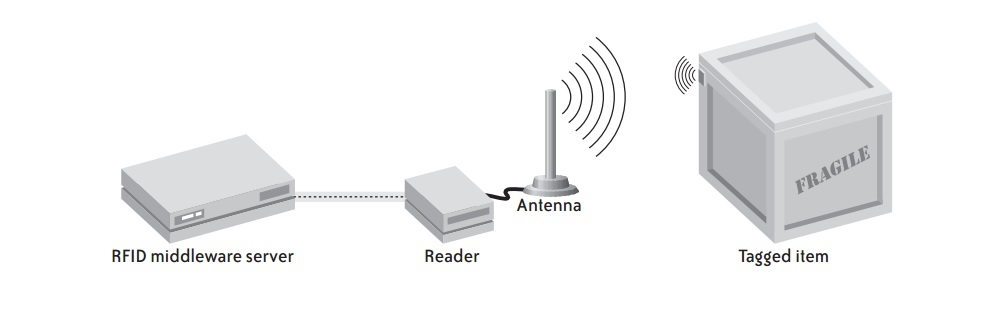
\includegraphics[width=0.6\linewidth]{rfidsys2}
		\caption{Sistema RFID típico, retirado de \cite{rfidbook}}
		\label{fig:rfidsys}
	\end{figure}
	
	Alguns dos benefícios do RFID são resumidos abaixo:
	\begin{itemize}
		\item Não há necessidade de alinhamento dos itens para leitura;
		\item Alta velocidade de inventário, pois vários itens podem ser lidos simultaneamente;
		\item Capacidade de identificar unicamente bilhões de itens;
		\item Variedade na forma das tags;
		\item Reusabilidade de tags.
	\end{itemize}
	
	\section{Evolução na adoção do RFID}
	De acordo com \cite{rfidbook}, podemos dividir o progresso de adoção do RFID em 5 períodos: \textit{Proprietary era}, \textit{Compliance era}, \textit{RFID-enable Enterprise era}, \textit{RFID-enable Industies era} e \textit{Internet of Things era}. A figura [\ref{fig:rfideras}] mostra quando algumas funções do RFID começaram ou vão começar a existir.
	
	\begin{figure}[h!]
		\centering
		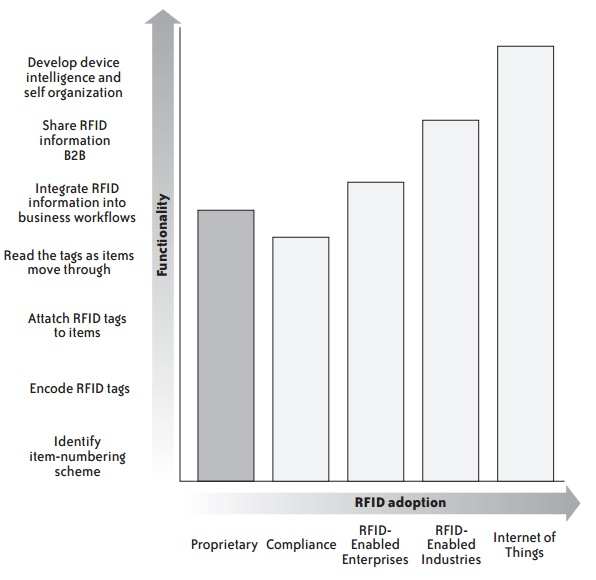
\includegraphics[width=0.6\linewidth]{rfideras}
		\caption{Evolução do RFID, retirado de \cite{rfidbook}}
		\label{fig:rfideras}
	\end{figure}
	
	No início (\textit{Proprietary era}), o RFID era usado para monitorar tipos particulares de itens e esta informação permanecia dentro das organizações que utilizavam o sistema. Isso fazia com que os sistemas fosse bastante específicos, dificultando bastante a comunicação entre parceiros de negócios. Alguns dos itens monitorados eram carros de trem, chassis de automóveis e gado leiteiro. Nesta época as tags ainda eram caras, logo estas eram reutilizadas sempre que possível. 
	
	Na \textit{Compliance era}, que representa o período atual, as empressas utilizam o RFID principalmente para garantir a interoperabilidade entre parceiros de negócios e agências regulatórias, não usando frequentemente os dados RFID para, por exemplo, aperfeiçoar alguns processos e melhorar a produtividade. A escassez de padrões e a falta de confiabilidade das novas tecnologias, impedem que as taga funcionem tão bem na prática como na época anterior.
	
	No futuro, teremos a \textit{The RFID-Enabled Enterprise era}, na qual as empresas começarão a utilizar as informações coletadas do RFID para o aprimoramento dos próprios processos. Isso será alcançado com a estabilização dos padrões e queda significativa dos custos. As empresas passarão a monitorar itens individuais ao invés de unidades de transporte, permitindo a coleta de mais informações sobre o processo. Entretanto, mesmo com a larga adoção interna do RFID, as empresas ainda precisam desenvolver os padrões necessários para permitir a troca de informações entre elas. 
	
	Em seguida teremos a \textit{The RFID-Enabled Industries era}, onde o uso de padrões RFID, redes de informação RFID, acordos de negócios e políticas de segurança e privacidade permitirão que empresas e cadeias de suprimentos troquem dados de forma segura e confiável entre si. Isso permitirá a descoberta de novas informações através do estudo  do grande volume de dados que estará disponível.   
	   
	Por fim, teremos a \textit{The Internet of Things era} que é atualmente uma previsão, na qual a ubiquidade da tecnologia RFID mudará a forma como vemos a relação entre informação, objetos físicos e localização. Por exemplo, a geladeira de nossa casa estará conectada à Internet e será capaz de ler a data de validade dos alimentos presentes e nos informar se algum deles já venceu. Além disso, ela poderá checar se algum produto está faltando e automaticamente realizar o pedido deste junto ao supermercado.
	
	A forma e velocidade com que os diversos tipos de usuários passarão por essas épocas não será feita de maneira uniforme. Atualmente, existem usuários que ainda estão na \textit{Proprietary era}, enquanto outros já estão começando a aplicar os conceitos da \textit{RFID-enabled Industries e Internet of Things}. Em algumas áreas, o RFID ainda nem começou a ser implementado.
	
	
	
	
	\newpage
	 \bibliographystyle{plain}
	 \nocite{*}
	 \bibliography{biblio_doc}
	 


\end{document}
\section{A Norma EPCGlobal}
\documentclass[a4paper,12pt,titlepage]{article}
\usepackage{palatino}
\usepackage{graphicx}
\usepackage{float}
\usepackage{amsmath}
\usepackage{caption}
\usepackage{subcaption}
\usepackage[margin=1.5cm,includefoot]{geometry}
\usepackage[utf8]{inputenc}
\usepackage{hyperref}
\usepackage{url}
\usepackage{listings}
\usepackage{xcolor}


\renewcommand*{\familydefault}{\sfdefault}
\usepackage[portuguese]{babel}


\begin{document}

\section{Introdução}	
	O uso da tecnologia RFID está em crescente expansão, principalmente em aplicações de Supply Chain Management (SCM), no qual saber a localização de cada item da cadeia produtiva é crucial para garantir maior eficácia e eficiência de todo um sistema. Devido essa crescente adoção do RFID, fica constatado que o surgimento de um conjunto de normas que visem à padronização das tecnlogias usadas seria algo natural de se acontecer. Imagine a situação em que uma grande empresa do setor de varejo se funda com outra do mesmo setor, sendo que ambas usam RFID para a localização dos produtos. Se, por exemplo, o formato das TAGs utlizadas pelas empresas forem diferentes, já teremos uma enorme dificuldade de integrar as informações oriundas de cada sistema. Para contornar esse tipo de problema, existe o \textbf{GS1}.
	
	O GS1 é uma organização internacional neutra e sem fins lucrativos, que desenvolve e mantém padrões para cadeias de demanda e suprimentos de diversos setores produtivos. Ele atua principalmente nas áreas de bens do consumo e varejo, saúde e transporte e logística. Algumas empresas que trabalham com o GS1 são: Carrefour, amazon, Google e Coca Cola. 	
	O GS1 foi fundado na década de 70 pelos líderes da indústria dos EUA, tendo com sua primeira atividade a criação do padrão de código de barras conhecido como \textbf{GS1 barcode}, o qual é largamente utilizado até hoje. Com os avanços da tecnologia e seu crescente uso, em 2004 o GS1 criou o primeiro padrão para o RFID.

	O padão GS1 é divido em três grupos: Identificar, Capturar e Compartilhar. 
	\begin{figure}[h!]
		\centering
		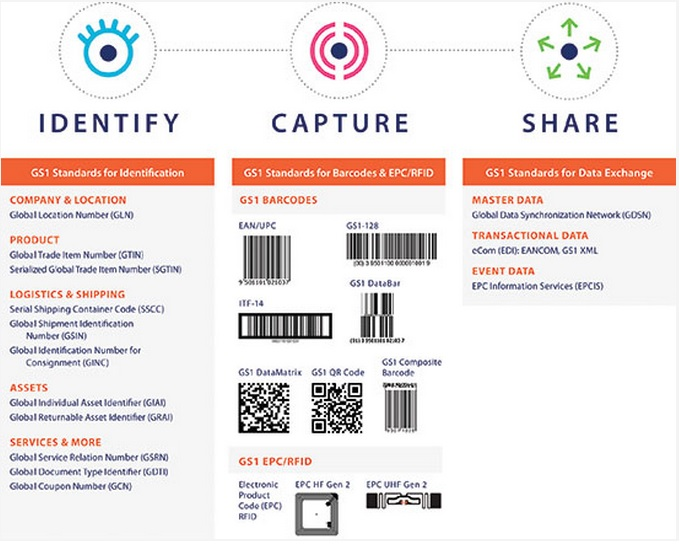
\includegraphics[width=0.7\linewidth]{gs1arch}
		\caption{Arquitetura do GS1}
		\label{fig:gs1arch}
	\end{figure}

	\paragraph{Identificar} Define códigos de identificação únicos que podem ser usados por um sistema de informação para se referir sem ambiguidade a qualquer tipo de produto.
	\paragraph{Capturar} Inclui definições de códigos de barra e RFID, além de especificar padrões para interfaces entre os elementos de software e hardware que se conectam às aplicações empresariais.
	\paragraph{Compartilhar} Define padrões para o formato dos dados trocados entre as aplicações e os clientes.     

	A norma voltada paraaplicações com RFID se enquadra no grupo "Capturar", e suas definições estão presentes no \textbf{EPCGlobal}.


\section{O padrão EPCGlobal}
	O padrão EPCglobal é uma iniciatia do GS1 para desevolver padrões voltados à indústria para o EPC, com o objetivo de dar suporte ao uso de RFID. Ele é divido em duas partes: \textbf{EPC/RFID Tags} e \textbf{EPCIS}. 
	
	O EPC (Electronic Product Code) é responsável por interligar o mundo do RFID com os códigos de barra do padrão GS1. Isso funciona da seguinte forma:
		\begin{figure}[h!]
			\centering
			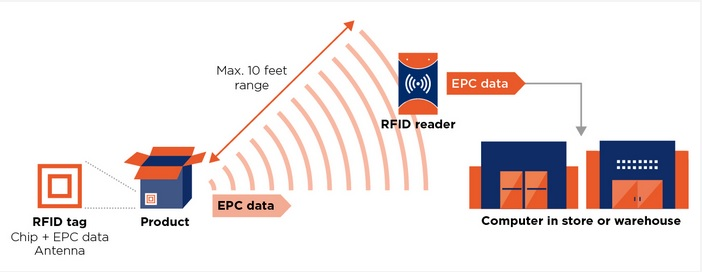
\includegraphics[width=0.5\linewidth]{epcrfid}
			\caption{Funcionamento do EPC}
			\label{fig:epcrfid}
		\end{figure}
	
	Cada produto contém um chip de memória contendo um EPC, o qual consiste de um número de série único. Em cada chip também há uma antena de rádio que transmite o EPC para um leitor RFID quando requisitado. Os dados capturados pelo leitor são então disponibilizados para os outros sistemas. A
	
	
	\begin{figure}[h!]
		\centering
		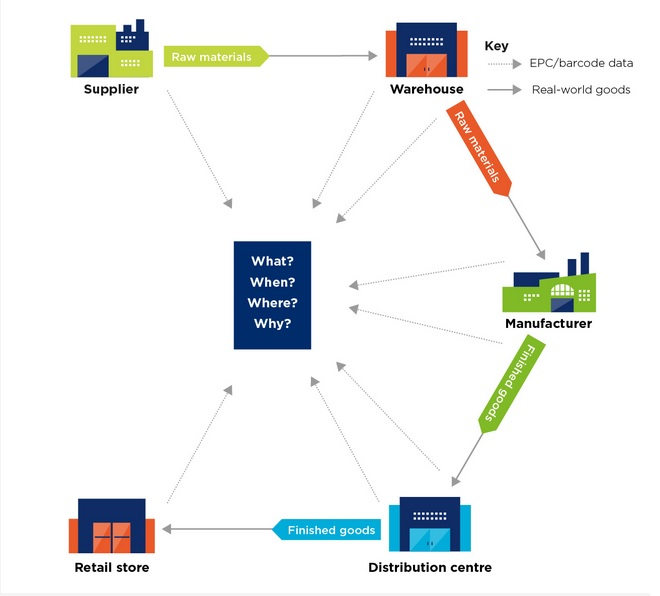
\includegraphics[width=0.5\linewidth]{epcis}
		\caption{Funcionamento do EPCIS}
		\label{fig:epcis}
	\end{figure}
	
	% Falar sobre o EPCIS
	O EPCIS (Electronic Product Code Information Services) é o padrão que habilita as empresas parceiras a compartilhar informações sobre o movimento físico e status dos produtos enquanto eles trafegam pela linha de suprimentos. Uma vez que os dados EPC são coletados, como na figura \ref{fig:epcrfid}, eles são disponibilizados à camada de negócios e todos que possuem acesso a este podem saber o histórico de movimento dos produtos. 
	
	\subsection{Arquitetura}

	O EPCGlobal define somente as interfaces, deixando as questões relativas à implementação sobre responsabilidade do usuário. Isso garante uma maior flexiblidade e alimenta o mercado de soluções em sistemas de informação para alcançar essa integração dos dados da cadeia produtiva. A figura \ref{fig:epcarc} apresenta um diagrama contendo a arquitetura básica de um sistema operando com a norma EPCGlobal.

	\begin{figure}[h!]
		\centering
		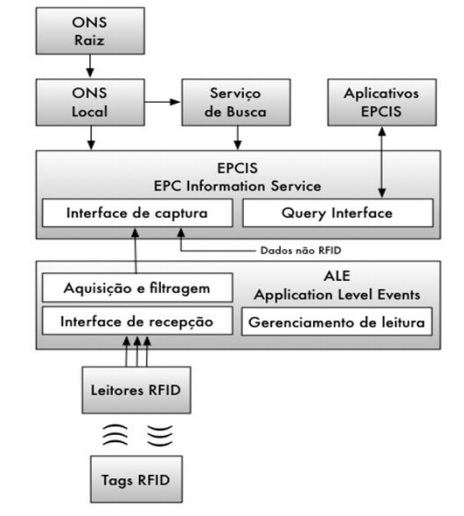
\includegraphics[width=0.5\linewidth]{epcarc}
		\caption{Arquitetura do EPCGlobal. Retirada de \cite{epcSobCug} }
		\label{fig:epcarc}
	\end{figure}
	
	A primeira camada contém os elementos necessários que permitem a identificação única de cada elemento da cadeia produtiva. Ela é composta pelo EPC, Tags e leitores RFID. 
	
	Entre os leitores RFID e as aplicações de captuda de dados está a interface ALE (Application Level Events). A ALE é uma camada de \textit{Middleware}, responsável por oferecer uma interface de alto-nível às aplicações capaz de agragar dados de diversos leitores, filtrá-los para remover redundâncias, como leituras múltiplas e não-desejadas e disponibilizá-los de maneira que as aplicações possam trabalhar mais facilmente com esses dados. Resumindo, a ALE é uma interface de pré-processamento de dados, que elimina a necessidade das aplicações de captura de dados lidarem com os aspectos de baixo nível da leitura de dados.
	
	Acima da ALE, temos o EPCIS. Esta é uma interface entre a captura de dados e as aplicações de nível empresarial. A troca de dados provenientes da ALE é feita através de mensagens XML padronizadas, tornando possível o uso do protocolo \textit{SOAP}. O compartilhamento destes dados para o público consumidor e/ou parceiros de negócios é definido pelas empresas, as quais decidem o grau com que elas irão disponiblizar essa informações. Este serviço é garantida pela \textit{Query Interface}, a qual integra os sistemas através de \textit{web services}, utilizando para isto os conceitos do \textit{SOA}. 
	
	Nas camadas mais superiores temos o Object Name Services (ONS), o qual é responsável por descobrir informações sobre um objeto com base no EPC. Para um dado EPC, a URL ou IP associado é pesquisado no banco de dados e os dados referentes àquele objeto podem ser econtrados e devolvidos à quem o requisitou. Ele funciona de maneira análoga a um servidor DNS, o qual traduz domínios em endereços IP.
	
\newpage

\bibliographystyle{plain}
\nocite{*}
\bibliography{biblio_doc}

		
\end{document}
\section{Conclusão}


\newpage
\bibliographystyle{plain}
\nocite{*}
\bibliography{biblio_doc}



\end{document}